%%
%% This is file `sample-sigconf.tex',
%% generated with the docstrip utility.
%%
%% The original source files were:
%%
%% samples.dtx  (with options: `all,proceedings,bibtex,sigconf')
%% 
%% IMPORTANT NOTICE:
%% 
%% For the copyright see the source file.
%% 
%% Any modified versions of this file must be renamed
%% with new filenames distinct from sample-sigconf.tex.
%% 
%% For distribution of the original source see the terms
%% for copying and modification in the file samples.dtx.
%% 
%% This generated file may be distributed as long as the
%% original source files, as listed above, are part of the
%% same distribution. (The sources need not necessarily be
%% in the same archive or directory.)
%%
%%
%% Commands for TeXCount
%TC:macro \cite [option:text,text]
%TC:macro \citep [option:text,text]
%TC:macro \citet [option:text,text]
%TC:envir table 0 1
%TC:envir table* 0 1
%TC:envir tabular [ignore] word
%TC:envir displaymath 0 word
%TC:envir math 0 word
%TC:envir comment 0 0
%%
%% The first command in your LaTeX source must be the \documentclass
%% command.
%%
%% For submission and review of your manuscript please change the
%% command to \documentclass[manuscript, screen, review]{acmart}.
%%
%% When submitting camera ready or to TAPS, please change the command
%% to \documentclass[sigconf]{acmart} or whichever template is required
%% for your publication.
%%
%%
\documentclass[sigconf]{acmart}
%%
%% \BibTeX command to typeset BibTeX logo in the docs
\AtBeginDocument{%
  \providecommand\BibTeX{{%
    Bib\TeX}}}

%% Rights management information.  This information is sent to you
%% when you complete the rights form.  These commands have SAMPLE
%% values in them; it is your responsibility as an author to replace
%% the commands and values with those provided to you when you
%% complete the rights form.
\setcopyright{acmlicensed}
\copyrightyear{2018}
\acmYear{2018}
\acmDOI{XXXXXXX.XXXXXXX}
%% These commands are for a PROCEEDINGS abstract or paper.
\acmConference[Conference acronym 'XX]{Make sure to enter the correct
  conference title from your rights confirmation emai}{June 03--05,
  2018}{Woodstock, NY}
%%
%%  Uncomment \acmBooktitle if the title of the proceedings is different
%%  from ``Proceedings of ...''!
%%
%%\acmBooktitle{Woodstock '18: ACM Symposium on Neural Gaze Detection,
%%  June 03--05, 2018, Woodstock, NY}
\acmISBN{978-1-4503-XXXX-X/18/06}


%%
%% Submission ID.
%% Use this when submitting an article to a sponsored event. You'll
%% receive a unique submission ID from the organizers
%% of the event, and this ID should be used as the parameter to this command.
%%\acmSubmissionID{123-A56-BU3}

%%
%% For managing citations, it is recommended to use bibliography
%% files in BibTeX format.
%%
%% You can then either use BibTeX with the ACM-Reference-Format style,
%% or BibLaTeX with the acmnumeric or acmauthoryear sytles, that include
%% support for advanced citation of software artefact from the
%% biblatex-software package, also separately available on CTAN.
%%
%% Look at the sample-*-biblatex.tex files for templates showcasing
%% the biblatex styles.
%%

%%
%% The majority of ACM publications use numbered citations and
%% references.  The command \citestyle{authoryear} switches to the
%% "author year" style.
%%
%% If you are preparing content for an event
%% sponsored by ACM SIGGRAPH, you must use the "author year" style of
%% citations and references.
%% Uncommenting
%% the next command will enable that style.
%%\citestyle{acmauthoryear}


%%
%% end of the preamble, start of the body of the document source.
\begin{document}

%%
%% The "title" command has an optional parameter,
%% allowing the author to define a "short title" to be used in page headers.
\title{Analysis of Communities formed in YouTube Comment Sections}

%%
%% The "author" command and its associated commands are used to define
%% the authors and their affiliations.
%% Of note is the shared affiliation of the first two authors, and the
%% "authornote" and "authornotemark" commands
%% used to denote shared contribution to the research.

\author{Thiago Amado Costa}
\email{thiago.amado@sga.pucminas.br}
\authornotemark[1]
\affiliation{%
  \institution{Pontifical Catholic University of Minas Gerais}
  \city{Belo Horizonte}
  \state{Minas Gerais}
  \country{Brazil}
}

\author{Humberto Torres Marques Neto}
\email{humberto@pucminas.br}
\authornotemark[2]
\affiliation{%
  \institution{Pontifical Catholic University of Minas Gerais}
  \city{Belo Horizonte}
  \state{Minas Gerais}
  \country{Brazil}
}


%%
%% By default, the full list of authors will be used in the page
%% headers. Often, this list is too long, and will overlap
%% other information printed in the page headers. This command allows
%% the author to define a more concise list
%% of authors' names for this purpose.
\renewcommand{\shortauthors}{Costa and Marques-Neto}

%%
%% The abstract is a short summary of the work to be presented in the
%% article.
\begin{abstract}
    YouTube is the largest video streaming platform on the web, attracting billions of users 
    daily who watch and engage with content through comments. 
    A significant portion of these users consist of children and teenagers, who frequently interact 
    with one another in the comment sections, forming active communities. 
    However, these communities can also experience negative interactions between users, 
    including instances of online bullying.
    To explore these communities, the YouTube Data API v3 was used to collect comments 
    from videos produced by creators targeting this demographic. These comments were used to construct 
    co-commenter networks.
    Topic modeling and sentiment analysis were then applied to gain deeper insights into the  
    content and dynamics within these communities.
\end{abstract}

%%
%% The code below is generated by the tool at http://dl.acm.org/ccs.cfm.
%% Please copy and paste the code instead of the example below.
%%
\begin{CCSXML}
<ccs2012>
   <concept>
       <concept_id>10010147.10010257.10010293</concept_id>
       <concept_desc>Computing methodologies~Machine learning approaches</concept_desc>
       <concept_significance>500</concept_significance>
       </concept>
 </ccs2012>
\end{CCSXML}

\ccsdesc[500]{Computing methodologies~Machine learning approaches}

%%
%% Keywords. The author(s) should pick words that accurately describe
%% the work being presented. Separate the keywords with commas.
\keywords{YouTube, Community Detection, Topic Modeling, Sentiment Analysis}
%% A "teaser" image appears between the author and affiliation
%% information and the body of the document, and typically spans the
%% page.

%%
%% This command processes the author and affiliation and title
%% information and builds the first part of the formatted document.
\maketitle

\section{Introduction}
YouTube has grown exponentially since its launch in 2005. With billions of users, it is now the 
largest video streaming platform on the web, and a major source of online entertainment content. 
As highlighted by \cite{app13064044}, many children and teenagers use the platform as an alternative to 
traditional entertainment sources, such as television, with the majority of their 
browsing time spent on YouTube. 

One way children and teenagers interact on the platform is through the comment section. 
This feature allows users to share their thoughts on the video, the content creator, and form online 
communities. These interactions can significantly impact their social development, behavior and 
attitudes. Additionally, the contrasting one-way relationship between users and content creators 
further amplifies this impact by creating emotional connections that shape how they experience social
media \cite{lozano2023social}. 
Furthermore, children's YouTube usage patterns are influenced by factors such as self-regulation 
abilities. These patterns not only affect their engagement with content but are also linked to 
emotional and behavioral problems \cite{kim2024temperament} .

The analysis of the communities formed in YouTube comments can provide valuable 
insights into the dynamics of user interactions, providing a deeper understanding of 
the platform's social ecosystem. This process involves identifying groups of users that share similar
behaviors, typically modeled as a graph, where nodes are represented by users and edges represent 
interactions, and unsupervised techniques as well as deep learning techniques are frequently employed 
to detect them \cite{nooribakhsh2024community}. For instance, a study utilized co-commenter networks 
to analyze suspicious commenter behaviors, leveraging network structural features and clustering 
methods to identify coordinated activities and behavioral similarities among channels \cite{shajari2023} .

The study by \cite{app13064044} demonstrates that many current developments focus on identifying
inappropriate content targeting young children. Advanced machine learning and deep learning 
techniques are being used to improve the detection of harmful videos, with the goal of enhancing 
children's safety on the platform. However, there is limited research focusing on the analysis of 
the social network communities formed on the comment section of YouTube creators who 
produce content aimed at children and teenagers.

This study aims to analyze the communities formed within the comment sections of YouTube creators who 
produce content aimed at children and teenagers, as well as the content of the comments themselves. 
To achieve this, 10 Brazilian YouTube creators were selected based on their 
subscriber count and total views. The analysis begins with the construction of a commenter dataset for 
each creator by collecting all comments from 50 videos. Subsequently, a co-commenter network is 
generated by linking users who commented on the same video. Graph metrics are then computed, and the 
Louvain Algorithm is applied to detect community structures within these networks. Additionally, the 
content of the comments is analyzed using Topic Modeling and Sentiment Analysis to gain further 
insights into their thematic and emotional characteristics. 
The results reveal notable community structures within the networks. Larger networks tend to exhibit 
weaker internal connections, while smaller communities show higher densities and clustering coefficients. 
Sentiment analysis indicates that positive comments typically express fan appreciation, whereas negative 
comments often reflect dissatisfaction with the content. 
Notably, it was possible to identify a specific community that exhibits negative sentiments due 
to possible organized activities, as well as signs of targeted advertising aimed at children and teenagers 
in another community. 

The remainder of this study is structured as follows. Section 2 reviews related work, highlighting 
prior research on community analysis, co-commenter networks, and sentiment analysis in the context 
of YouTube and children's content. Section 3 details the methodology, including data collection, 
co-commenter network construction, community detection using the Louvain Algorithm, and the application 
of topic modeling and sentiment analysis. Section 4 presents the results of the analysis, focusing 
on the community structures identified, their characteristics, and insights from sentiment and topic 
modeling. Finally, Section 5 summarizes key findings, discusses limitations, and proposes directions for 
future research.

\section{Related Work}

% Comunidade
A social network community can be defined as a set of members of that specific network that interact
with each other, similar to real-world communities but in an online environment.
These online communities are shaped based on how users interact on each platform, and the analysis
of such communities can uncover hidden relationships between users and how they engage \cite{nooribakhsh2024community}.

A recent research by \cite{kirdemir2023} uses community analysis to investigate coordinated 
inauthentic campaigns on YouTube, focusing on characterizing suspicious behaviors through a 
multi-step analysis of engagement trends and co-commenter networks. These co-commenter networks are
built by connecting two commenters if they commented on the same video.
By analysing these co-commenter networks and channel engagement trends, they were able to identify
patterns indicative of manipulation, such as increasing views paired with decreasing subscribers, 
and highlight channels exhibiting coordinated 
commenting behaviors. In \cite{shajari2023}, the authors follow this methodology to
explore the problematic behaviors of commenters on YouTube, specifically focusing on "commenter mobs" 
that manipulate engagement metrics to distort public perception. 
By analyzing 20 targeted channels through social network analysis, the research fills gaps in 
understanding how suspicious commenter activities boost engagement, which has been insufficiently 
addressed in prior literature. Employing a co-commenter network model and clustering techniques, 
the study identifies distinct groups with varying levels of suspiciousness and highlights collusion 
among commenters across channels. Key findings reveal central figures driving discussions and 
coordinated efforts to amplify specific narratives, suggesting these channels significantly contribute 
to the spread of misinformation. 

% TODO: falar que e de um canals so
With a similar methodology, the study by \cite{hussain2018analyzing} investigates
disinformation tactics used on a specific conspiracy theory channel, distinguishing its approach by 
focusing on user engagement patterns rather than just spam detection. Data was collected using the 
YouTube Data API, monitoring metrics like views, likes, dislikes, and comments, revealing patterns 
indicative of potential manipulation. The analysis identified two commenter groups, peripheral and 
core, with the second group exhibiting higher instances of inorganic behaviors. A co-commenter network 
analysis revealed clusters around specific conspiracy topics and identified bot-like and spam actions. 

% Polarizacao / Topic Modeling
In \cite{shekar2021}, the authors investigate the prevalence and nature of abusive comments on YouTube, 
particularly focusing on the impact of hate speech on users, especially teenagers, by utilizing 
exploratory data analysis and topic modeling. 
The study employed Latent Dirichlet Allocation (LDA) for topic modeling and sentiment analysis using 
the TextBlob library to assess the emotional tone of comments. Findings revealed that certain 
YouTubers received significantly harsher comments, with varying sentiment levels indicating the 
need for interventions to protect young creators from severe online harassment. 
The study concludes by recommending measures such as disabling comments on particularly abused 
videos and emphasizes the importance of understanding the dynamics of cyberbullying.

% kids
In the context of children's content on YouTube \cite{app13064044}, machine learning and deep learning 
techniques are used to analyze video, audio, and user comments to detect inappropriate 
material. These methods often rely on natural language processing for text analysis and computer 
vision for visual content detection. 
Despite recent advancements, the challenge of accurately detecting inappropriate content targeted at 
this demographic using machine learning and deep learning approaches still persists.

This study differs from the previously mentioned works, by focusing specifically on the co-commenter 
networks formed in the comment sections of YouTube creators who produce content aimed at children and teenagers. 
While prior research has explored co-commenter networks to detect suspicious behaviors, coordinated activities, 
and abusive language, these studies have primarily targeted general or adult-oriented content. 
Additionally, research on children's content has largely concentrated on detecting inappropriate 
material within videos rather than analyzing user interactions. By combining community detection 
through the Louvain Algorithm with Topic Modeling and Sentiment Analysis, this work provides a 
perspective on the thematic and emotional dynamics within these communities, 
addressing a gap in understanding the social interactions surrounding child-focused content on YouTube.

\section{Methodology}

This section outlines the methodology employed, which is divided into three main phases: 
data collection, community analysis, and comment analysis, as illustrated in Figure~\ref{fig:methodology}. 
The data collection phase describes the process of gathering comments from selected YouTube channels 
using the YouTube Data API v3. The community analysis phase explains the construction of co-commenter 
networks, the application of the Louvain Algorithm for community detection, and the computation of 
graph metrics to characterize these networks. Finally, the comment analysis phase details the use of 
BERTopic for topic modeling and XLM-RoBERTa for sentiment analysis to uncover thematic and emotional 
patterns within the comments. Each phase is described in detail to provide a comprehensive overview 
of the methodological steps taken to analyze user interactions in YouTube comment section.

\begin{figure*}[t!]
    \centering
    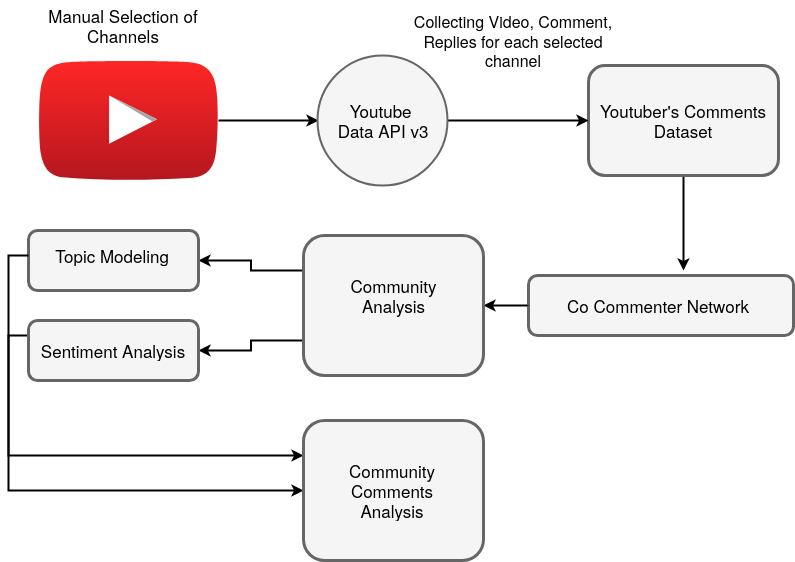
\includegraphics[keepaspectratio,width=0.9\textwidth]{./imgs/tcc_methodology.png}
    \caption{Methodology}
    \label{fig:methodology}
\end{figure*}

\subsection{Data Collection}

Initially, the YouTube Data API v3 was used to gather comprehensive channel metadata for a group of YouTube creators. 
Ten creators were selected through Viewstats\footnote{https://www.viewstats.com/}, an analytics platform 
that facilitates ranking the most viewed channels by country and category.
and chosen based on the size of their subscriber base, total view count, and content type, as summarized in 
Table~\ref{tab:youtubers}.

\begin{table}[ht!]
\centering
\caption{YouTubers with Subscribers and Views}
\label{tab:youtubers}
\resizebox{\columnwidth}{!}{
\begin{tabular}{cccl}
\toprule
\textbf{YouTuber}        & \textbf{Subscribers}    & \textbf{Total Views}       & \textbf{Content Type }      \\ 
\midrule
Felipe Neto              & 46,800,000             & 18,171,376,895        & Entertainment, vlogs        \\ 
Enaldinho                & 40,000,000             & 18,009,391,826        & Entertainment, vlogs        \\ 
Natan por Aí             & 24,800,000             & 16,409,135,985        & Entertainment, vlogs        \\ 
Rezendeevil              & 33,800,000             & 13,686,976,806        & Entertainment, vlogs        \\ 
Robin Hood Gamer         & 21,500,000             & 11,309,149,204        & Gaming (Minecraft, Roblox)  \\ 
Brancoala                & 13,100,000             & 9,897,577,900         & Family vlogs, Games         \\ 
AuthenticGames           & 20,100,000             & 8,967,486,579         & Gaming (Minecraft)          \\ 
Camila Loures            & 15,600,000             & 5,509,570,500         & Lifestyle vlogs             \\ 
Geleia                   & 10,200,000             & 3,207,064,265         & Gaming (Minecraft)          \\ 
CadresPlayer             & 8,640,000              & 2,640,042,941         & Gaming (Minecraft)          \\ 
\bottomrule
\end{tabular}}
\end{table}

Subsequently, the video IDs and titles for 50 videos from each channel were retrieved. 
Finally, a dataset of user-generated comments and replies was constructed by aggregating all comments 
and their replies associated with the selected videos. Additional contextual information, such as 
the video titles and the number of likes each comment received, was also collected. 
The number of comments collected per channel ranges approximately 11,000 to 43,000.


\subsection{Community Analysis}

To analyze the communities that emerge within each YouTuber's comment section, the datasets constructed 
in the previous phase are used to construct the co-commenter networks. Each commenter is connected to
another if they commented on the same video, and the weight of the edge is increased if they commented
on more than one video together. To maintain only the stronger connections, we filtered out co-commenters
who commented on less than 10 videos together, as done by \cite{shajari2023} and \cite{kirdemir2023}. 

To identify the communities of each co-commenter network the Louvain Algorithm was used. This 
algorithm was chosen because of its high efficiency and performance on real-world networks
without ground truth, as shown by \cite{YOU2020104822}.

Following the method developed by \cite{kirdemir2023}, a set of metrics were computed 
for each co-commenter network, including average degree, number of nodes and edges, average coefficient,
modularity, coverage, the number of communities identified with the Louvain Algorithm. Graph clique 
metrics were also computed, including the number of maximal cliques that have at least five members, 
average clique size, median clique size, average degree of clique members, average clustering coefficient
of clique members. To discover the similarities between the chosen channels, these metrics were used
with KMeans and Hierarchical Clustering, along with Principal Component Analysis to reduce the complexity
while maintaining important features.

\subsection{Comments Analysis}

To further understand user behavior, we implement
topic modeling and sentiment analysis. For the topic modeling phase, we employ the BERTopic model 
(\cite{bertopic2022}), while the sentiment analysis is conducted using the multilingual 
XLM-roBERTa-base model(\cite{barbieri-etal-2022-xlm}). 
Initially, the comments are processed and cleaned, masking user handles to preserve anonymity,
removing emojis, links and stop words.
Then, topic modeling is utilized to extract themes associated with the communities identified in the 
previous phase. Finally, the sentiment analysis model evaluates the polarity of the content, 
offering deeper insights into the emotional tone of the discussions and facilitating a more 
comprehensive analysis of the communities.

\section{Results}

In this section, the results are shown and analyzed. 
Considering that a modularity value above 0.3 is a good indicator of significant
community structures in a network \cite{PhysRevE.70.066111}, the Louvain algorithm successfully 
identified significant community structures in all the YouTube creator's co-commenter networks.
The KMeans and Hierarchical Clustering methods were applied with the community metrics described, 
with the reduced complexity of the Principal Component Analysis (PCA). 
Both methods identified 5 distinct clusters, as can be seen in Figure ~\ref{fig:kmeans_hierarchical}.

\begin{figure}[hbt!]
    \centering
    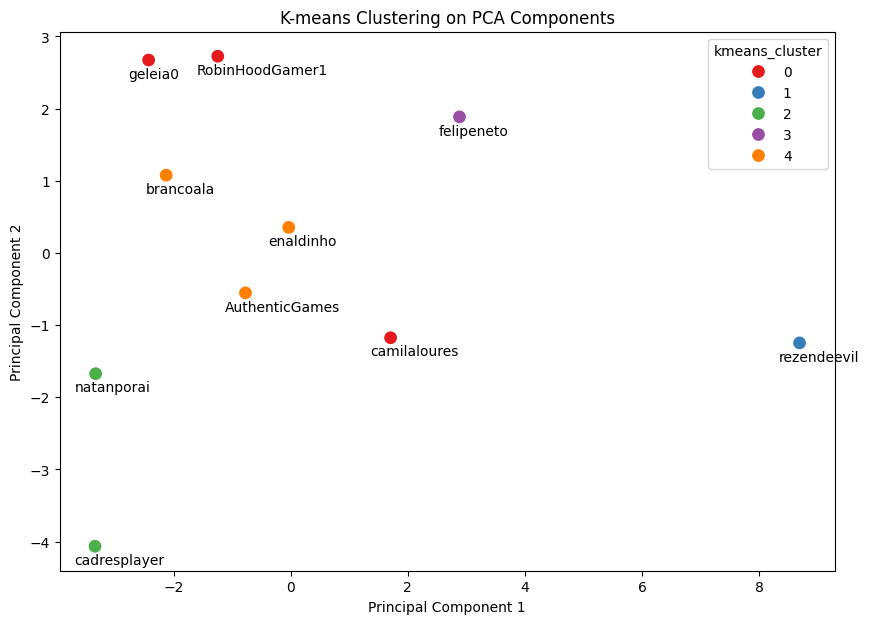
\includegraphics[width=\linewidth]{./imgs/KMeans_PCA.png}
    \vspace{0.5cm} % Add some vertical space between the images
    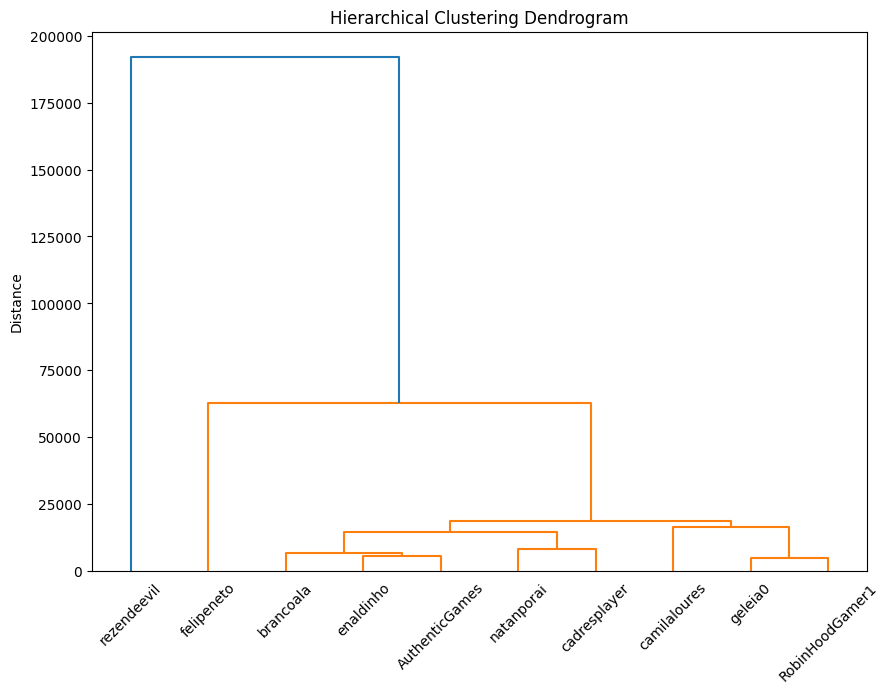
\includegraphics[width=\linewidth]{./imgs/Hierarchical_clustering.png}
    \caption{KMeans and Hierarchical Clustering}
    \label{fig:kmeans_hierarchical}
\end{figure}


The most distinguishable channels are on clusters 1 (Rezendeevil) and 3 (Felipe Neto). 
Both creators had very large co-commenter networks, with Rezendeevil's network having 13,808 
nodes and 149,033 edges, and Felipe Neto having 24,987 nodes and 125,165 edges.
The creator Rezendeevil had the lowest modularity (0.52) but the highest average degree (21.5), 
along with the greatest number of maximal cliques and the largest average clique size.
This indicates that both creators have high interconnected and engaged communities. The higher average
degree indicates that Rezendeevil's followers are more engaged than Felipe Neto's, while the higher
modularity score shows that Felipe Neto's community structure is more distinct.
This can be seen through Figure~\ref{fig:rezendeevil_comm} and Figure ~\ref{fig:felipeneto_comm}, 
with each community colored.

A per community sentiment analysis showed that most comments on Rezendeevil's videos were labeled as 
positive by the XLM-roBERTa-base model, which is consistent with a highly engaged community of fans.
Most positive comments focus on the video content, specific individuals featured, or compliments directed toward the creator. 
Through topic analysis, a recurring theme labeled 
"quero" was identified, with comments such as "Eu quero" and "Eu quero muito uma." 
(translated as "I want" or "I really want one").
These comments predominantly come from members of communities 5 and 6, characterized by higher density 
values (0.15) and lower conductance metrics (0.07) relative to other communities
Additionally, these communities exhibit lower clustering coefficients, a pattern observed across all communities.
A more detailed investigation of the videos receiving these comments could reveal potential 
signs of direct or implicit advertising aimed at children and teenagers.

In contrast to Rezendeevil, Felipe Neto had more negative comments than positive comments. 
By analyzing the polarity per community, it was possible to identify that community 12, 
that has the highest percentage of negative comments (55.3\%), is also the community with the highest clustering 
coefficient of approximately 0.23 , lowest conductance of approximately 0.06 and highest density 
of 0.21. This may indicate a close-knit organized community that frequently comment on the 
same content spreading negative and hateful comments. 
Topic Modeling also shows recurring themes labeled "Brasil", "Hipocrisia" 
("Hypocrisy"), "Dinheiro, Pobres" ("Money, Poor"), with comments such as 
"é tanta burrice por metro quadrado é um absurdo como tem gente que acredita nestas hipocrisias" 
("it's such stupidity per square meter, it's absurd how many people believe in these hypocrisies."),
"Esse Felipe merda é uma das desgracas que so existe aqui no Brasil, ..." 
("This Felipe piece of trash is one of the disasters that only exists here in Brazil, ..."). 
Figure ~\ref{fig:felipeneto_comments} provides a word cloud visualization of these comments.
The term 'user' is used as a placeholder to mask instances where one commenter mentions another user's 
name.
The other communities had lower densities, lower average clustering coefficients and higher values 
of conductance. These communities displayed a wider variety of topics and a higher number of positive 
comments compared to community 12. 

\begin{figure}[hbt!]
    \centering
    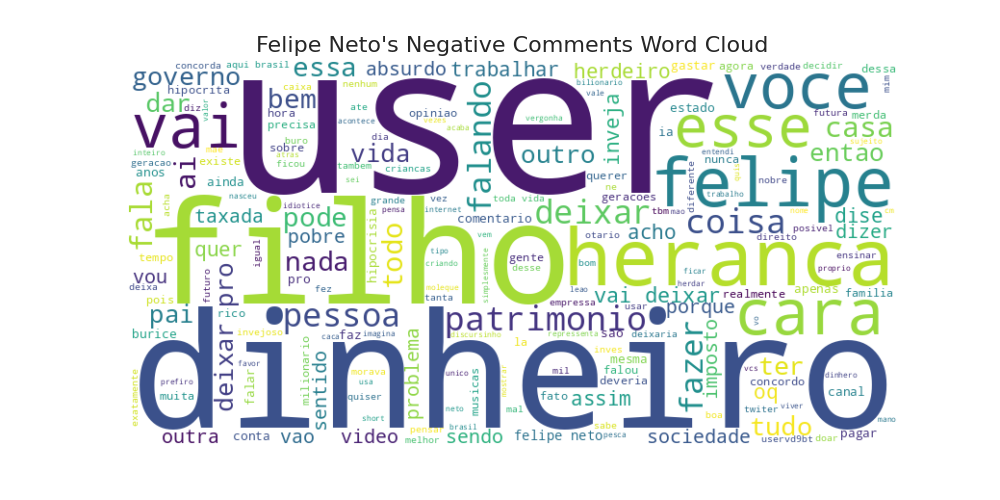
\includegraphics[keepaspectratio,width=\linewidth]{./imgs/felipeneto/negative_comments.png}
    \caption[width=\textwidth]{Felipe Neto's negative comments word cloud}
    \label{fig:felipeneto_comments}
\end{figure}

\begin{figure}[t]
    \centering
    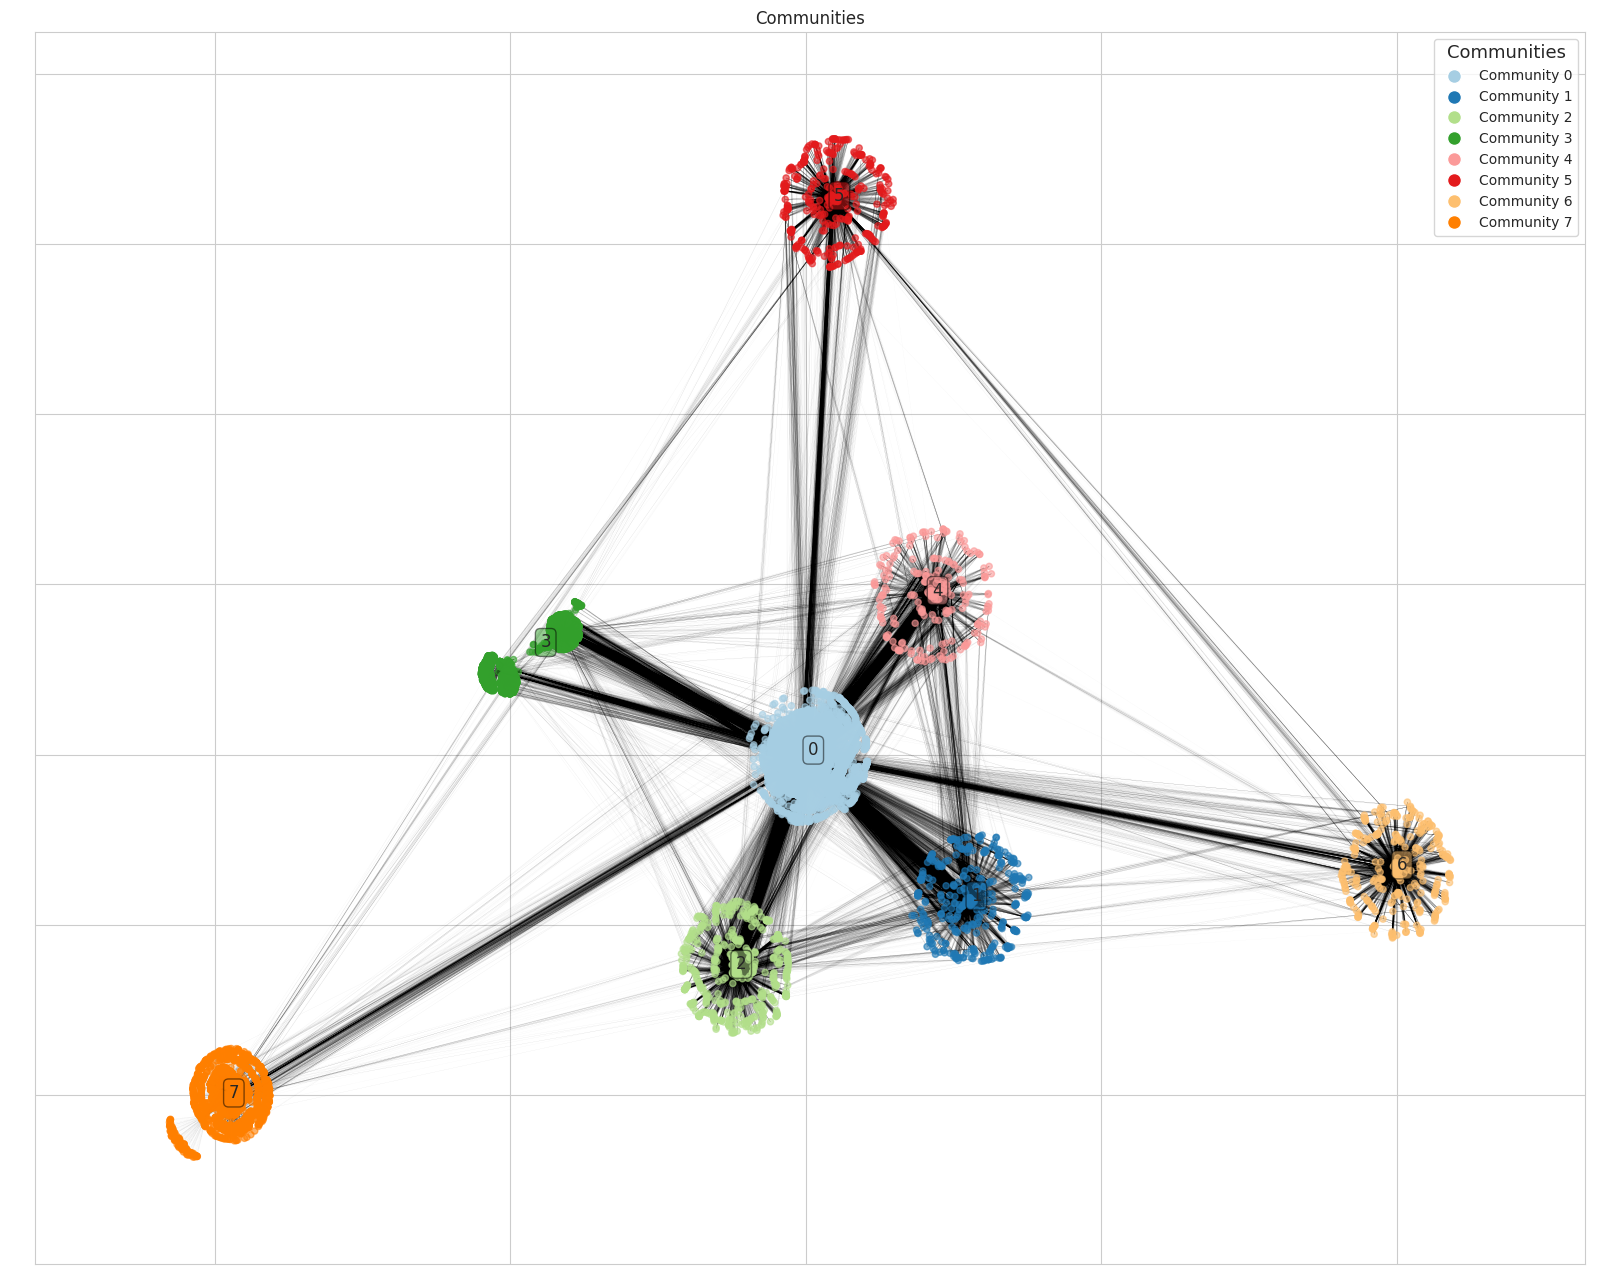
\includegraphics[keepaspectratio,width=\linewidth]{./imgs/rezendeevil/communities.png}
    \caption[width=\textwidth]{Rezendeevil's Communities}
    \label{fig:rezendeevil_comm}
\end{figure}

\begin{figure}[t]
    \centering
    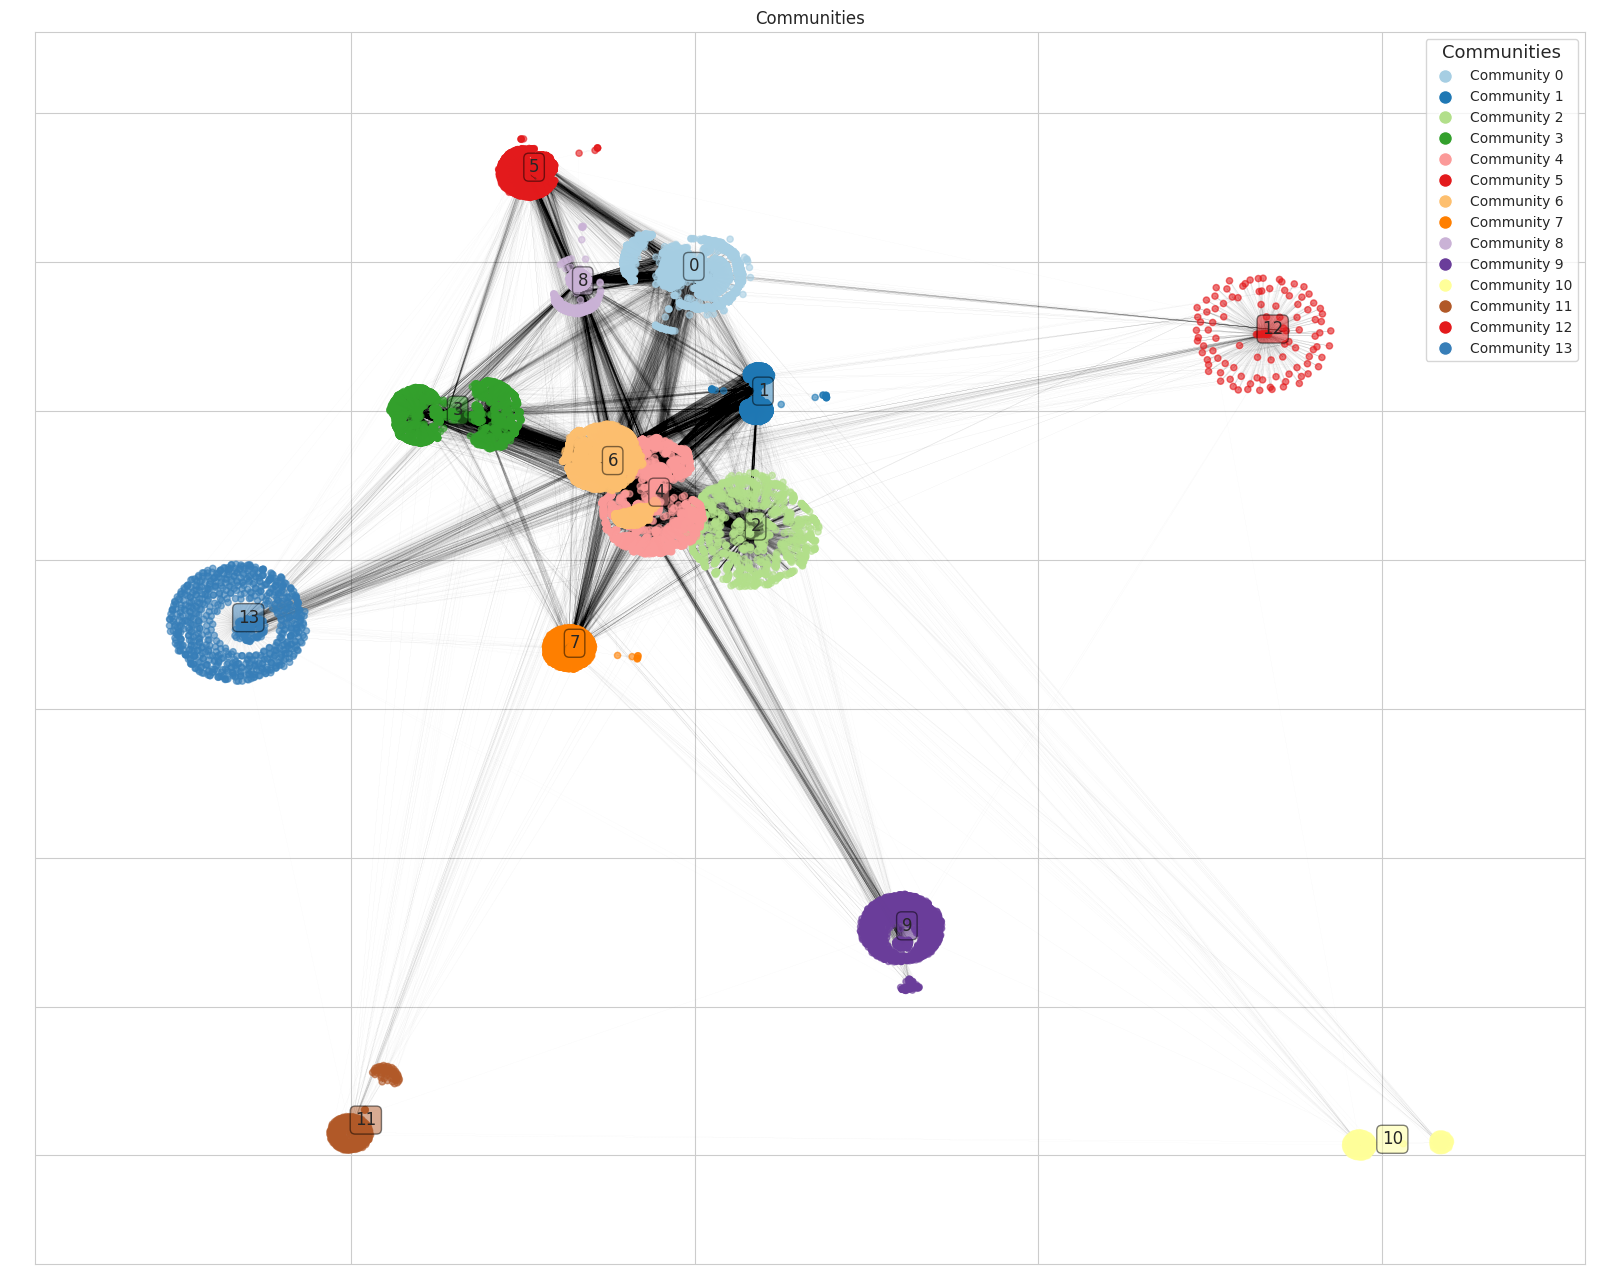
\includegraphics[keepaspectratio,width=\linewidth]{./imgs/felipeneto/communities.png}
    \caption[width=\textwidth]{Felipe Neto's Communities}
    \label{fig:felipeneto_comm}
\end{figure}

Cluster 2 represents creators with smaller, tightly-knit networks with stronger internal connections,
which suggests that users within their communities frequently interact with each other but not much across
different subgroups. Topic Modeling shows that topics related to fan appreciation dominate across 
all comunities, with comments like "Te amo Cadres" ("I love you Cadres"), "Oi Natan eu sou teu fan"
("Hi Natan, I'm your fan"). 
The analysis of both creators' communities with the highest proportion of negative comments showed that
while their communities can be critic about their content, they are not entirely hostile.
Most negative feedback arises from unmet expectations or dissatisfaction with specific content, 
with comments like "Não faz isso Natan voce pode morrer sem ar" ("Don't do this, Natan, you could suffocate")
or "Natan faz algo melhor que isso" ("Natan, do something better than this"). 
For Cadresplayer, many criticisms focused on the creator's voice, with topics frequently labeled by
the keywords "voice","strange","AI","different". This was reflected in comments such as "Cadres sua voz 
mudou, está parecendo um robô" ("Cadres, your voice has changed, it sounds like a robot").
For both creators, the communities with the highest proportion of negative comments have varying numbers
of clustering coefficient, density and conductance.

The networks of Camila Loures, Robin Hood Gamer, and Geleia0 in Cluster 0 exhibit 
moderately engaged networks, with significant differences in their community dynamics. 
All three creators have networks characterized by high modularity values (Geleia0: 0.90, Robin Hood Gamer: 
0.84, Camila Loures: 0.64), indicating well-defined subgroups, though Camila Loures’s network is 
more interconnected with fewer communities (7) compared to the more fragmented networks of Robin Hood Gamer 
(24 communities) and Geleia0 (31 communities). 
The average degree is highest for Camila Loures (12.44), suggesting higher 
interaction levels among her commenters, while the clustering coefficients are low across all creators, 
indicating sparse local connectivity within communities. 

In terms of topics and sentiment polarity, Camila Loures's 
audience engages positively with lifestyle content, though criticism arises around repetitive 
video formats.
The analysis of the creator's less positive communities revealed negative feedback on 
video styles or lack of originality ("Essa temporada ta ruim demais muito chata", "This season is really bad, very boring"), 
as well as neutral comments with content requests ("Você poderia fazer um vídeo mais interativo com os fãs.", 
"You could make a more interactive video with fans").
These communities demonstrated higher density values, lower conductance metrics, and a significantly 
elevated average degree (approximately 25, compared to less than 10 in all other communities). 
However, they exhibited a low average clustering coefficient.

Robin Hood Gamer follows a similar pattern of feedbacks. His fans engage positively around Minecraft videos, 
with many supporting comments from fans. 
The analysis of the less positive communities also revealed 
negative feedback related to content, often focused on content quality, as well as suggestions for future 
content improvements. However, these communities did not show significant differences compared to the rest of 
the creator's communities, also showing varying values of clustering coefficient, density and conductance.
Geleia0 shows a similar pattern to Robin Hood Gamer, but with emphasis on the communities with the highest proportion of
negative comments (44.8\% and 38.3\%) with comments often expressing frustration, insults, or dissatisfaction with the content 
or creators. These comments frequently include abusive language, criticism of creators' personalities 
or actions, and expressions of anger across different themes. Examples include 
"O dream é um monstro matou o próprio pet que raiva" ("Dream is a monster; he killed his own pet, how infuriating."), 
"Aaaaaaa o geleia é muito burroooooooo que ódio" ("Aaaaaaa Geleia is so dumb, how hateful."), 
"Nao foi justo ele tirou o messi porque ele nao gosta da argentina" ("It wasn't fair, he took out Messi because he doesn't like Argentina").
Figure ~\ref{fig:geleia_comments} provides a word cloud visualization of these comments.  

\begin{figure}[hbt!]
    \centering
    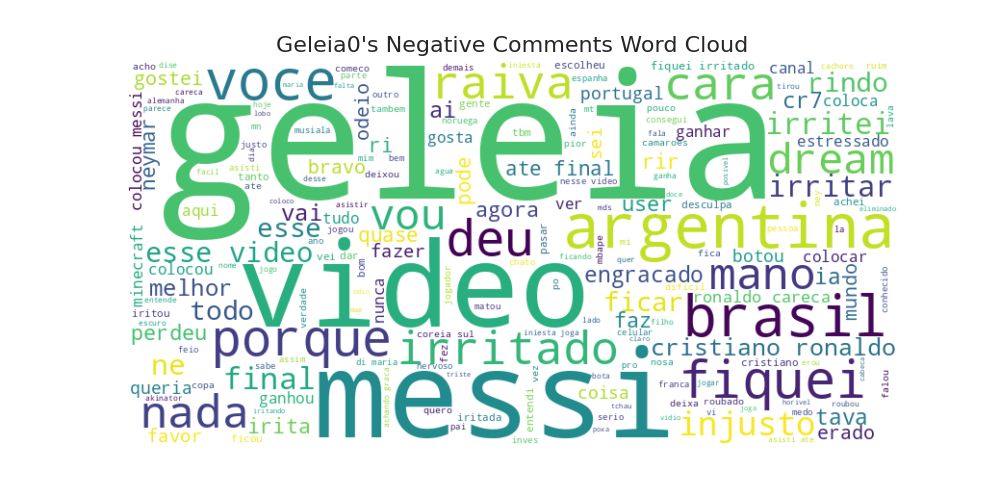
\includegraphics[keepaspectratio,width=\linewidth]{./imgs/geleia/negative_comments.png}
    \caption[width=\textwidth]{Geleia0's negative comments word cloud}
    \label{fig:geleia_comments}
\end{figure}

Cluster 4 represents creators with moderately sized networks that show similar community dynamics and 
thematic engagement, exhibiting network structures with node counts ranging from 11,000 to 12,000 and 
edge counts varying between 26,000 and 37,000. 
The creators in this cluster (Enaldinho, AuthenticGames, and Brancoala) 
have networks characterized by high modularity values (ranging from 0.75 to 0.86), 
though their clustering coefficients are low, reflecting sparse local connectivity within communities. 
Enaldinho has 14 communities, AuthenticGames has 20, and Brancoala has 19, which shows varying levels 
of audience fragmentation. Topic Modeling revealed the same pattern of content requests, negative feedback
over repetitive content and fan appreciation.
For all creators of this cluster, the communities with the highest proportion of negative comments showed
varying numbers of average clustering coefficient, density and conductance.

Overall, the analysis of YouTube co-commenter networks revealed distinct patterns of community 
structure, engagement, and thematic focus across the identified clusters. 
Each cluster exhibits unique characteristics based on graph metrics, sentiment polarity and topic modeling.
Across all co-commenter networks, the communities identified with the Louvain algorithm showed varying 
numbers of clustering coefficient, density and average degree. Table~\ref{tab:network_analysis} shows
the main metrics used per cluster.

\begin{table}[h!]
\caption{Network Characteristics by Cluster}
\label{tab:network_analysis}
\resizebox{\columnwidth}{!}{
\begin{tabular}{cccccl}
\toprule
\textbf{Cluster} & \textbf{Nodes} & \textbf{Edges} & \textbf{Avg Degree} & \textbf{Modularity}  \\ 
\midrule
0             & 8,800-19,900  & 54,800-72,000      & 7.2-12.4 & 0.64-0.90 \\ 
1             & 13,808        & 149,033            & 21.58    & 0.52  \\ 
2             & 2,700-5,300   & 5,200-13,000       & 3.7-4.8  & 0.78-0.83 \\ 
3             & 24,987        & 125,165            & 10.01    & 0.65  \\ 
4             & 11,000-12,800 & 26,000-37,500      & 4.5-5.9  & 0.72-0.87  \\ 
\bottomrule
\end{tabular}}
\end{table}

Across all clusters, neutral comments dominate, reflecting passive engagement or constructive feedback.
While positive sentiments typically reflect fan appreciation, 
negative responses generally stem from unmet expectations or frustration with repetitive content, with 
occasional hateful and targeted comments. 
Larger communities serve as broader hubs with weaker internal connections,
possibly with users that don't often interact with others.

Within the networks of clusters 0, 2 and 4, smaller communities generally show higher densities and 
clustering coefficients compared to larger ones. Overall, polarity within these communities is generally 
non-hostile, with exceptions that are sporadically distributed across communities. 
Analysis of the most negative communities reveals diverse characteristics: 
while some display more elevated density and clustering coefficient values, 
others exhibit lower values. Complementing this sentiment analysis, topic modeling provides additional insights,
for example fans of Cadresplayer expressed dissatisfaction with the creator's voice, 
describing it as robotic, while Geleia0's fans engaged in discussions on sports-related themes.

In contrast, the analysis of Cluster 3's network identified a distinct group disseminating negative 
comments directed at the creator and other users, with topic modeling revealing recurring themes within 
these interactions. Meanwhile, the analysis of Cluster 1's network with topic modeling highlighted 
potential indicators of direct or implicit advertising.

\section{Conclusion}

This study analyzed the communities formed in the comment sections of YouTube creators who produce 
content aimed at children and teenagers. By leveraging co-commenter network analysis, community detection 
with the Louvain Algorithm, topic modeling, and sentiment analysis, the research uncovered significant 
insights into the structure, engagement, and thematic dynamics of these online communities.

The findings highlighted the existence of distinct community structures within YouTube comment sections. 
By grouping channels into clusters, the analysis allowed for a detailed comparison of the similarities 
and differences across these networks. Topic modeling and sentiment analysis revealed consistent 
patterns across all creators: positive comments were primarily associated with fan appreciation, 
neutral comments indicated passive engagement, and negative comments often reflected unmet expectations 
or dissatisfaction. 

However, exceptions were noted. For instance, in Cluster 3 the network analysis revealed a distinct 
community spreading negative comments, with higher values of clustering coefficient and density, and low conductance.
This pattern was unique to Cluster 3, in other networks, communities with similar network metrics 
did not necessarily correspond to higher levels of negativity. 
Communities with high negativity were found across clusters 0, 2 and 4 both in groups with similar network 
characteristics to Cluster 3's community (high density and clustering coefficient) and in those with 
lower network metric values. 
    
This research demonstrates the value of examining social interactions in YouTube comments through the 
combined application of community analysis, topic modeling, and sentiment analysis. Future studies would benefit 
from exploring alternative community detection algorithms, analyzing larger datasets spanning 
multiple videos and channels, investigating overlapping community structures, and extending the analysis to 
different social media platforms. This expanded scope would provide deeper insights into 
user behavior and community dynamics, ultimately contributing to the development of a  safer online 
environment for children and teenagers.

\begin{acks}
To my family and friends, for their love and support, and to the professors, for their guidance 
and teachings throughout this journey.
\end{acks}

%%
%% The next two lines define the bibliography style to be used, and
%% the bibliography file.
\bibliographystyle{ACM-Reference-Format}
\bibliography{sample-base}


%%
%% If your work has an appendix, this is the place to put it.
% \appendix


\end{document}
\endinput
%%
%% End of file `sample-sigconf.tex'.
